\documentclass{article}

% if you need to pass options to natbib, use, e.g.:
%     \PassOptionsToPackage{numbers, compress}{natbib}
% before loading neurips_2021

% ready for submission
\usepackage[preprint]{neurips_2021}

% to compile a preprint version, e.g., for submission to arXiv, add add the
% [preprint] option:
%     \usepackage[preprint]{neurips_2021}

% to compile a camera-ready version, add the [final] option, e.g.:
%     \usepackage[final]{neurips_2021}

% to avoid loading the natbib package, add option nonatbib:
% \usepackage[nonatbib]{neurips_2021}




\usepackage[utf8]{inputenc} % allow utf-8 input
\usepackage[T1]{fontenc}    % use 8-bit T1 fonts
\usepackage[colorlinks = true, 
		    linkcolor = blue,
		    urlcolor  = blue,
            citecolor = blue,
            anchorcolor = blue]{hyperref}       
% hyperlinks
\usepackage{url}            % simple URL typesetting
\usepackage{booktabs}       % professional-quality tables
\usepackage{amsfonts}       % blackboard math symbols
\usepackage{nicefrac}       % compact symbols for 1/2, etc.
\usepackage{microtype}      % microtypography
\usepackage{xcolor}         % colors
\usepackage{natbib}
\usepackage[pdftex]{graphicx}
\usepackage{siunitx} % Required for alignment
\sisetup{
  round-mode          = places, % Rounds numbers
  round-precision     = 2, % to 2 places
}
	

\bibliographystyle{unsrtnat}

\title{Clustering Spotify: How diverse is popular music?}




% The \author macro works with any number of authors. There are two commands
% used to separate the names and addresses of multiple authors: \And and \AND.
%
% Using \And between authors leaves it to LaTeX to determine where to break the
% lines. Using \AND forces a line break at that point. So, if LaTeX puts 3 of 4
% authors names on the first line, and the last on the second line, try using
% \AND instead of \And before the third author name.


\author{%
  Dominik Glandorf\\
  Matrikelnummer 6007407\\
  \texttt{dominik.glandorf@student.uni-tuebingen.de} \\
  \And
  Felix D. Gross\\
  Matrikelnummer 6001480\\
  \texttt{fel.gross@student.uni-tuebingen.de} \\
}

\begin{document}

\maketitle

\begin{abstract}
{In this work we investigate if popular music is less diverse. From Spotify, metadata of 28,195 tracks was collected, notably the audio features, to assess the cliché of contemporary pop music being all the same. To evaluate variability, a visual analysis via PCA and F-tests were conducted. The 2D plot showed already a visible difference between pop and non-pop songs. The analysis of variance confirmed that the variability across certain audio features is indeed less in pop music when compared to non-pop music, thereby confirming our initial hypothesis. Consequently, we discussed issues of sampling bias and imbalanced data.}
  
\end{abstract}

\section{Introduction}

Music is one of the oldest and most valued forms of communication and is therefore of particular interest. Yet, its underlying structure has been eluded systematic analysis until recently. Comparing numerous features across thousands of songs was too much data to handle with traditional methods of analysis. Accelerated computing and freely accessible databases allow now for systematic inquiry of music. Thus it is only now possible to hold common clichés about music proof to the real world data.

One of these clichés is, that pop music is all the same and less diverse then non-popular music \citep[see for example][]{serra2012measuring}. Thus, our hypothesis is, that the variability of pop music is smaller, then the one observed in non-popular music.

Since Spotify is the worlds most used music streaming platform, it promises to be representative for global music listening taste.

% What are "pop songs"? What do we mean by variability? What is an audio feature of a track? Declare them as our features and popularity as the label of interest, (terminology of machine learning, psychology terms could be included i.v., d.v.). Why do we think that this measures diversity? Maybe then outline of the subsequent sections 

\section{Method}

\subsection{Sample}
The music metadata was obtained from the Spotify Web API \citep{spotifyAPIdocu}. In order to compile our sample, the search endpoint was queried in the following way: For each possible single Latin letter and two letter combination the first 50 search results were stored. This led to a potential number of \(27 * 26 * 50 =\) 35,100 results. After eliminating duplicates in the result lists, the total sample encompassed \(N_{total} =\) 28,195 songs. The list of songs was then augmented by the results from the audio features endpoint. We concentrated on danceability, energy, liveness, loudness, speechiness, acousticness, instrumentalness, tempo, valence and key, as they allow for easy and intelligible interpretations of the lofty term variability % explain each feature, based on their documentation, % add why we dropped key as a non-ordinal (categorical) feature
The specific meaning of each of these features can be obtained from the documentation of the Spotify API \citep{spotifyAPIdocu}[table, or still explain here?]. In addition to these features, which provide information about the internal make-up of the song, Spotify offered also a "popularity" feature. A value between 0 and 100 is assigned to each song, with 100 being the most popular. We used this feature to assign our sample to two groups: the pop songs and the non-pop songs. An inspection of the current charts and music played regularly in the radio, led us to use a popularity threshold of 90. Using this limit, the \(n_{pop} = 70\) most popular songs were assigned to the pop song group and the remainder \(n_{non pop} = 28,125\) to the non pop song group.

\subsection{Analysis}
To ensure data quality and get a first idea of the data, we started the analysis by graphically and numerically checking the distributions of our audio features and the popularity in the sample. A correlogram served to see if we expect linear dependencies between our features and the label or between features.

As stated above, we were interested in the variability of pop songs compared to the remainder. Hence, we first employed an exploratory and visual approach before running statistical tests. In order to search for an underlying structure in the audio features and to be able to get a first impression of the data as a whole we decided to do a dimensionality reduction via Principal Component Analysis (PCA). We decided against a stochastic neighbor embedding such as t-SNE since we only had 9 dimensions and believed in a global structure that might not be preserved by those methods. To be able to plot the principal components we chose the two components that explained the most variance. Since the PCA is agnostic to the grouping we indicated them in the visualization, in hope to see a structure.

Independently of the results of the data exploration, we planned to conduct a two sample variance comparison on each audio feature \citep{snedecor1989}. Based on our hypothesis, that did not comprised mean differences in the two groups but rather variance differences, the weapon of choice was a classical F-test for independent samples. Because we conducted multiple F-tests we used the conservative instrument of the Bonferroni correction to decide for significance. To further assess our estimation quality we did a bootstrap sampling from both groups and calculated the variance quotient, i.e. the F-statistic for each of them. According to  here \cite{kruschke2014doing}
we calculated the 95\% HDI (highest density interval) that contains the 95\% of variance ratios that we most often encountered in the bootstrap procedure .

\subsection{Results}

\begin{figure}
  \centering
  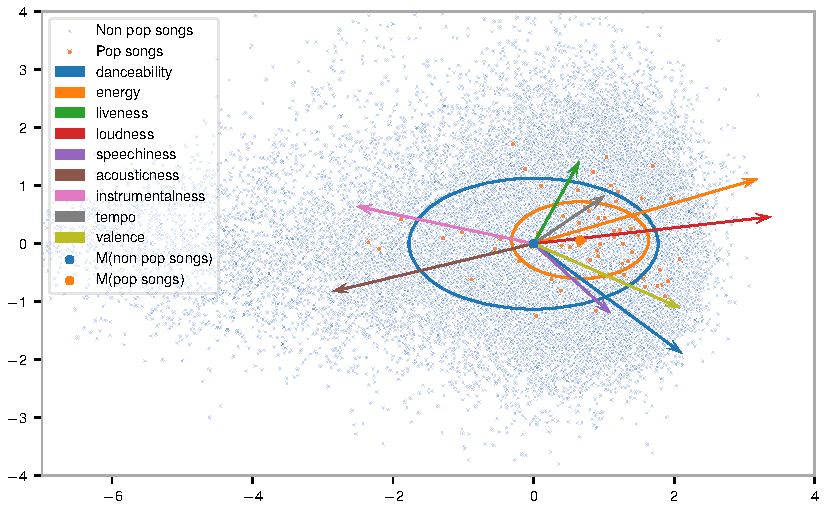
\includegraphics[]{../fig/001_pca.pdf}
  \caption{The projected sample on the first two principal components}
\end{figure}

\begin{figure}
  \centering
  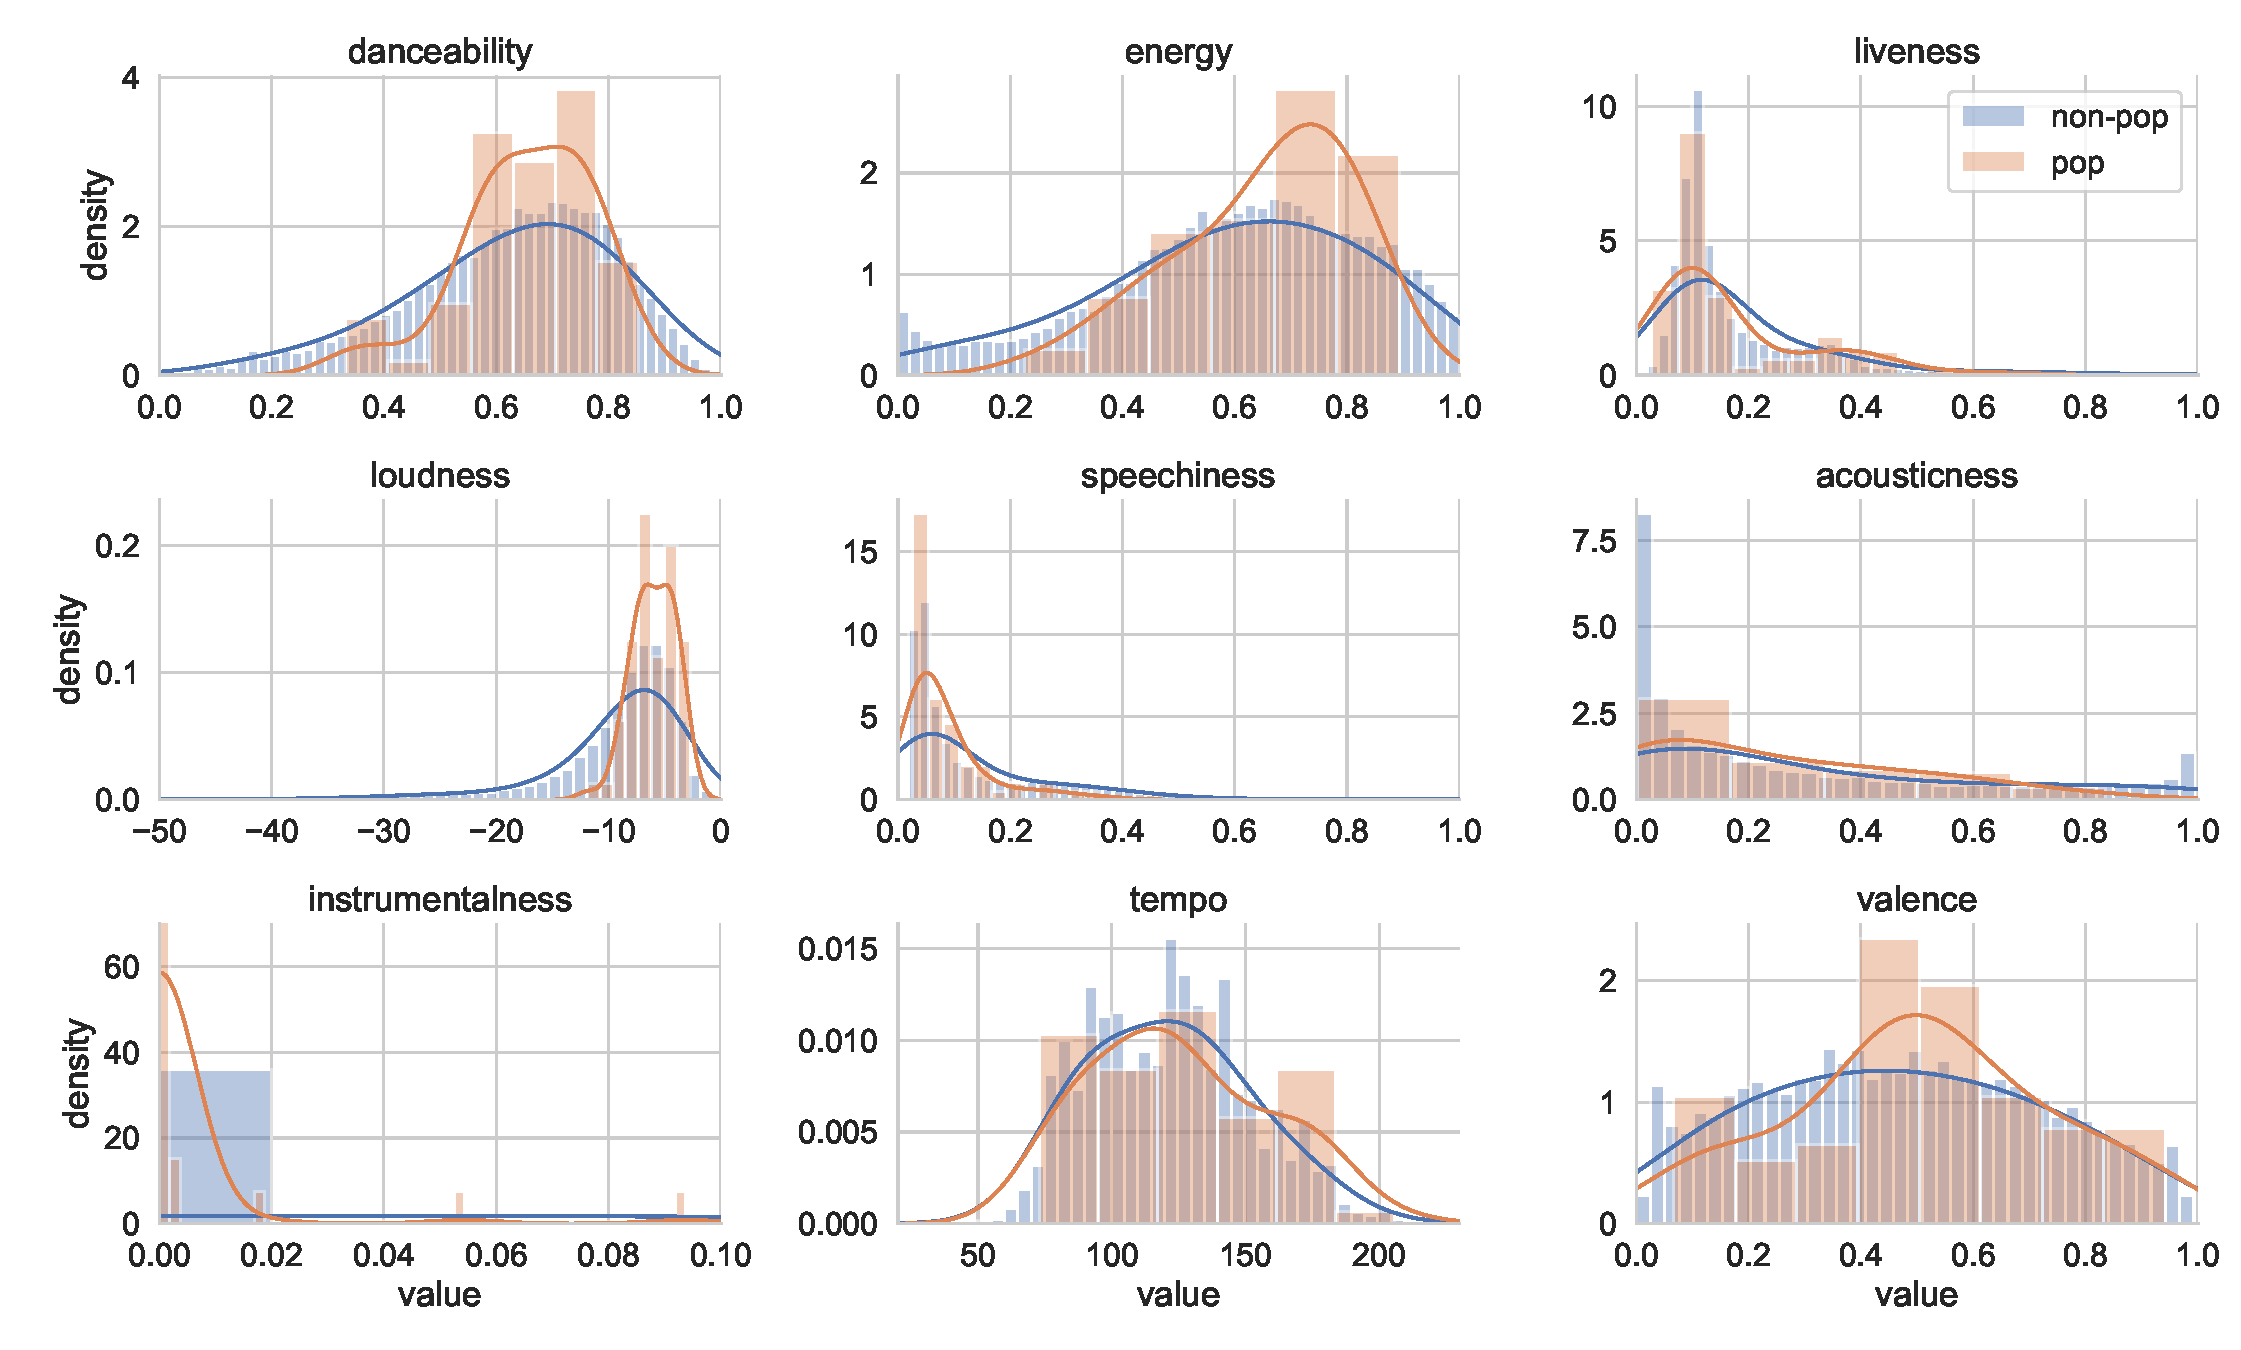
\includegraphics[width=1\linewidth]{../fig/002_variances.pdf}
  \caption{Variances.}
\end{figure}

\begin{table}[h!]
  \caption{Significance-test}
  \label{sample-table}
  \centering
  \begin{tabular}{lllc}
    \toprule
      &                     &  Results    &\\
    \cmidrule(r){3-4}
    No.     & Feature     & F-value & Range\\
    \midrule
    1 & danceability        &  2.50** &\\
	2 & energy              &  2.26** &\\
	3 & liveness            &  1.23   &\\
	4 & loudness            &  9.27** &\\
	5 & speechiness         &  3.57** &\\
	6 & acousticness        &  1.80*  &\\
	7 & instrumentalness    &642.00** &\\
	8 & tempo               &  0.83   &\\
	9 & valence             &  1.21   &\\
    \bottomrule
  \end{tabular}
\end{table}


% no real correlation
% non-normal distribution of some features

% use tueplots

% PCA results

% Variance tests results
Six of the tested features  % which audio features are significant?

\subsection{Discussion}
The variance of six of the evaluated nine features was significantly less in the pop-music group, if compared to the non-pop music group, hereby supporting our hypothesis of pop music being all the same.  
The unusual high variance difference 


nine features between 


% is our sampling strategy adequate?


% imbalanced data, justify why it is inherent in our analysis and why we think that our results are still not biased by this imbalance
 It resulted  to be a suitable size for a hit parade, most of Spotify's own hit play-lists consist out of 50 songs, 
-other features
-other pop treshold (continous descibtion)
% consider different markets/cultures, Spotify is heavily based to Western music, suggestion for further research, replicate our analysis for each countries charts

% Future research idea: Check over time, if there is a change or manifestation in variance ratios.

% Look at the output and repair capitalization and 
\bibliography{library.bib}

\end{document}
